Wolfenstein 3D is a game that needs little introduction. Released in May 1992, it layed down the fundation of First Person Shooter achieving instant legendary status. Universaly acclaimed, the beautiful graphics, crisp digitalized sounds, engaging musics and oustanging game design made its engine sing. Within a year more than 100,000 units had been sold bringing game and a little bit of fortune to the game studio producing it: id Software.\\
\\
The many fans did not stop at completing the game. They started to reverse engineer the game. Within a few months the assets formats were well known and people released modified version\footnote{Better know as \emph{mods}} with altered graphics, sounds effects, music and maps. The core of the game however, the secrets of its speed remained mostly unknown.\\
\\
It remained a well guarded secret for obvious reasons. A good game engine was and still is considered the main asset of a game company. As a mean to outperform competitior it is paramount to hide the algorithms and datastructure.\\
\\
But a faction within id Software did not see things that way. Instead of advocating what commercial common sense would dicate, they wanted to embrace player's enthousiasm and fully open the source code to the public. Internal discussuion [ASK JOHN HOW HARD IT WAS. After many internal debate, id Software did the unthinkable: On July 21, 1995 they posted a zip archive on ftp.idsoftware.com containing source code and instructions to build an executable.\\
\\

 \begin{fancyquotes}
   Programming is not a zero-sum game. Teaching something to a fellow programmer doesn't take it away from you. I'm happy to share what I can, because I'm in it for the love of programming.\\
   \\
\textbf{John Carmack - Programmer}
 \end{fancyquotes}
\\
Pessimist people could have forecasted the demise of a company so foolish to give away its technology for free. Instead it made id Software an icon. People that loved programming could relate to a company dedicated to the Right Thing.\\
\\
Sharing their knowledge despite common sense elevated id Software and contributed to build an aura of contributors.\\
\\
Opening the source code also allowed their software to live and run well after the hardware it was running on died. Twenty years after the release of Wolfenstein 3D and Doom, you can still play the game on anything with a CPU and some RAM. From a super computer to a cellphone.\\
\\
An unexpected side effect of releasing the source is that it created a window back in time. To read it is like being back in 1992. As the techincal writer on fabiensanglard.net I originally thought i would never take a cool at this old thing. But when out of curiosity I took a peek, I could not stop reading. I was mezmerized by how hard it was to program back in the days. I realized the Tour de Force Wolfenstein 3D was: The IBM PC had been designed for office work, not gaming. It is misleading to look at a mips graph such as Figure ref{fig:game_console_vs_PC}\\
\\
\begin{figure}[H]
\centering
  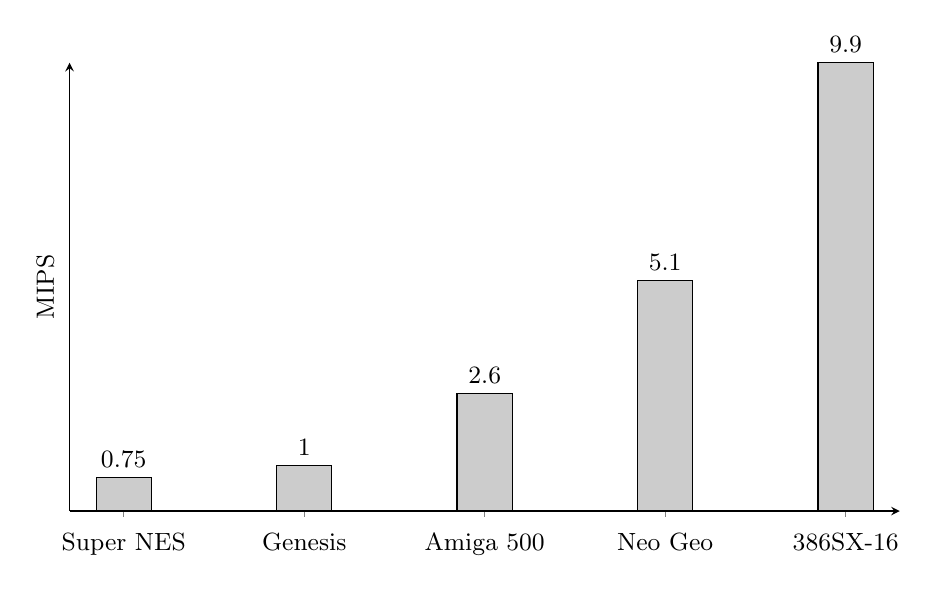
\begin{tikzpicture}[font=\small]
    \begin{axis}[
      width=1.0\textwidth,
      height=0.6\textwidth,
      ybar=6pt,
      bar width=20pt,
      ylabel={MIPS},
      ymin=0,
      ytick=\empty,
      xtick=data,
      axis x line=bottom,
      axis y line=left,
      enlarge x limits=0.075,
      symbolic x coords={Super NES,Genesis,Amiga 500,Neo Geo,386SX-16},
      xticklabel style={anchor=base,yshift=-\baselineskip},
      nodes near coords={\pgfmathprintnumber\pgfplotspointmeta}
    ]
      \addplot[fill=black!20,draw=black] coordinates {
        (Super NES,0.75)
        (Genesis,1)
        (Amiga 500,2.6)
        (Neo Geo,5.1)
        (386SX-16,9.9)
      };
    \end{axis}
    
   \end{tikzpicture}
   \caption{Game Console Vs PC.} \label{fig:game_console_vs_PC}
 \end{figure}
\\
And conclude that because PC were so powerful, it would be "easy" to write a game, and not that great of an achievement to make a worlwide hit. But Game console were designed around animation. They all had coprocessors and Graphic Unit relying on tile engine. Animating a sprite on the screen was just about to update it's {x,y} coordinates.\\
\\
\\
\\
But game console were specifically build and designed to produce 60 frames per seconds animations. Among other things they all had co-processors powering a tile-based system. PCs were sitting on the antipod: Built around a single processor and a framebuffer (a structure were every pixel has to be populated individually) the machine was not designed for gaming, it was intended to crunch integers and display static content.\\
\\
This is where the root of my admiration for Wolfenstein 3D lies: id Software achieved the unthinkable by building a game engine able to display pseudo 3D at 30 frames per seconds on an IBM PC.\\
\\
This book "raison d'etre" is to expose how limited and unwelcoming the hardware was and how the software managed to not only workaround the many limitations but sometimes managed to turn them into an advantage.\\
\\
I saw beauty in how the hardware was repurposed of used in unexpected ways. You had to be driven by passion to program games on those things. Even the engineers building the the hardware would have said that what id Software was trying to achieve was not what the machines were meant to do. This is where the true beauty of Wolfenstein 3D is: For every obstacles, the id Software team found a way to not only circumvent the limitations but often turn them into advantages.

\bigskip

 \textbf{\underline{Disclaimer :}} The description that follows is technical and will appeal mostly to programmers. If you are more into the human aspect of game programming I would recommend instead to read David Kushner’s chef d’oeuvre: “Masters of Doom: How Two Guys Created an Empire and Transformed Pop Culture”.
This book tries to give a detailed story of how Wolfenstein 3D was done. It is divided in three parts reviewing the hardware, the team and the software.